% !TeX program = pdfLaTeX
\documentclass[12pt]{article}
\usepackage{amsmath}
\usepackage{graphicx,psfrag,epsf}
\usepackage{enumerate}
\usepackage{natbib}
\usepackage{textcomp}
\usepackage[hyphens]{url} % not crucial - just used below for the URL
\usepackage{hyperref}
\providecommand{\tightlist}{%
  \setlength{\itemsep}{0pt}\setlength{\parskip}{0pt}}

%\pdfminorversion=4
% NOTE: To produce blinded version, replace "0" with "1" below.
\newcommand{\blind}{0}

% DON'T change margins - should be 1 inch all around.
\addtolength{\oddsidemargin}{-.5in}%
\addtolength{\evensidemargin}{-.5in}%
\addtolength{\textwidth}{1in}%
\addtolength{\textheight}{1.3in}%
\addtolength{\topmargin}{-.8in}%

%% load any required packages here


\usepackage{color}
\usepackage{fancyvrb}
\newcommand{\VerbBar}{|}
\newcommand{\VERB}{\Verb[commandchars=\\\{\}]}
\DefineVerbatimEnvironment{Highlighting}{Verbatim}{commandchars=\\\{\}}
% Add ',fontsize=\small' for more characters per line
\usepackage{framed}
\definecolor{shadecolor}{RGB}{248,248,248}
\newenvironment{Shaded}{\begin{snugshade}}{\end{snugshade}}
\newcommand{\AlertTok}[1]{\textcolor[rgb]{0.94,0.16,0.16}{#1}}
\newcommand{\AnnotationTok}[1]{\textcolor[rgb]{0.56,0.35,0.01}{\textbf{\textit{#1}}}}
\newcommand{\AttributeTok}[1]{\textcolor[rgb]{0.77,0.63,0.00}{#1}}
\newcommand{\BaseNTok}[1]{\textcolor[rgb]{0.00,0.00,0.81}{#1}}
\newcommand{\BuiltInTok}[1]{#1}
\newcommand{\CharTok}[1]{\textcolor[rgb]{0.31,0.60,0.02}{#1}}
\newcommand{\CommentTok}[1]{\textcolor[rgb]{0.56,0.35,0.01}{\textit{#1}}}
\newcommand{\CommentVarTok}[1]{\textcolor[rgb]{0.56,0.35,0.01}{\textbf{\textit{#1}}}}
\newcommand{\ConstantTok}[1]{\textcolor[rgb]{0.00,0.00,0.00}{#1}}
\newcommand{\ControlFlowTok}[1]{\textcolor[rgb]{0.13,0.29,0.53}{\textbf{#1}}}
\newcommand{\DataTypeTok}[1]{\textcolor[rgb]{0.13,0.29,0.53}{#1}}
\newcommand{\DecValTok}[1]{\textcolor[rgb]{0.00,0.00,0.81}{#1}}
\newcommand{\DocumentationTok}[1]{\textcolor[rgb]{0.56,0.35,0.01}{\textbf{\textit{#1}}}}
\newcommand{\ErrorTok}[1]{\textcolor[rgb]{0.64,0.00,0.00}{\textbf{#1}}}
\newcommand{\ExtensionTok}[1]{#1}
\newcommand{\FloatTok}[1]{\textcolor[rgb]{0.00,0.00,0.81}{#1}}
\newcommand{\FunctionTok}[1]{\textcolor[rgb]{0.00,0.00,0.00}{#1}}
\newcommand{\ImportTok}[1]{#1}
\newcommand{\InformationTok}[1]{\textcolor[rgb]{0.56,0.35,0.01}{\textbf{\textit{#1}}}}
\newcommand{\KeywordTok}[1]{\textcolor[rgb]{0.13,0.29,0.53}{\textbf{#1}}}
\newcommand{\NormalTok}[1]{#1}
\newcommand{\OperatorTok}[1]{\textcolor[rgb]{0.81,0.36,0.00}{\textbf{#1}}}
\newcommand{\OtherTok}[1]{\textcolor[rgb]{0.56,0.35,0.01}{#1}}
\newcommand{\PreprocessorTok}[1]{\textcolor[rgb]{0.56,0.35,0.01}{\textit{#1}}}
\newcommand{\RegionMarkerTok}[1]{#1}
\newcommand{\SpecialCharTok}[1]{\textcolor[rgb]{0.00,0.00,0.00}{#1}}
\newcommand{\SpecialStringTok}[1]{\textcolor[rgb]{0.31,0.60,0.02}{#1}}
\newcommand{\StringTok}[1]{\textcolor[rgb]{0.31,0.60,0.02}{#1}}
\newcommand{\VariableTok}[1]{\textcolor[rgb]{0.00,0.00,0.00}{#1}}
\newcommand{\VerbatimStringTok}[1]{\textcolor[rgb]{0.31,0.60,0.02}{#1}}
\newcommand{\WarningTok}[1]{\textcolor[rgb]{0.56,0.35,0.01}{\textbf{\textit{#1}}}}

% Pandoc citation processing

\usepackage{booktabs}
\usepackage{longtable}
\usepackage{array}
\usepackage{multirow}
\usepackage{wrapfig}
\usepackage{float}
\usepackage{colortbl}
\usepackage{pdflscape}
\usepackage{tabu}
\usepackage{threeparttable}
\usepackage{threeparttablex}
\usepackage[normalem]{ulem}
\usepackage{makecell}
\usepackage{xcolor}

\begin{document}


\def\spacingset#1{\renewcommand{\baselinestretch}%
{#1}\small\normalsize} \spacingset{1}


%%%%%%%%%%%%%%%%%%%%%%%%%%%%%%%%%%%%%%%%%%%%%%%%%%%%%%%%%%%%%%%%%%%%%%%%%%%%%%

\if0\blind
{
  \title{\bf Identify Lesions within CT Scans Using Convolutional Neural Networks}

  \author{
        Graham Chickering \\
    \\
      }
  \maketitle
} \fi

\if1\blind
{
  \bigskip
  \bigskip
  \bigskip
  \begin{center}
    {\LARGE\bf Identify Lesions within CT Scans Using Convolutional Neural Networks}
  \end{center}
  \medskip
} \fi

\bigskip
\begin{abstract}
Convolutional Networks are a specific type of Neural Networks that have
shown to be particularly effective at being able to identify distinct
objects within images. This technique can be used to identify different
types of anomalies, such as lesions, within medical images as well as
detect other sorts of tumors or cancers. In theory this type of network
is designed based on how the human brain works and the idea that
multiple levels of neurons are connected together in order to detect and
identify images. In practice though, running and training these types of
neural networks can be very computationally expensive and require large
amounts of memory and processing capabilities if working with a very
large dataset. Especially when working in R which has limited memory
capabilities, trying to run and train this type of model can be very
slow and ineffective. Thanks to developments in cloud computing and
distributed data processing engines such as Google Cloud Storage and
Apache Spark, being able to run and train these types of models within R
can become much faster and more efficient when trying to analyze large
amounts of data. While there is more work to be done, this project shows
how to create an infrastructure that efficiently stores data and trains
these models when working with the R Studio Environment.
\end{abstract}

\noindent%
{\it Keywords:} Convolutional Neural Networks, Apache Spark, Google Cloud Storage,
Lesions, Healthcare
\vfill

\newpage
\spacingset{1.45} % DON'T change the spacing!

\hypertarget{introduction}{%
\section{Introduction}\label{introduction}}

It has been estimated that roughly 80\% of healthcare data is
unstructured data, which can come in the form of videos, sensor data,
images, or text. Although hospitals and researchers used to have a hard
time extracting insights from this type of data, with the recent
advances that have been made in data science and handling big data, this
has created new application areas within the healthcare industry in
sectors such as genomics, drug trials, predicting patient health, and
medical imagery. Medical imaging research in particular has made
significant progress recently with researchers being able to use
different machine learning algorithms to detect different types of
lesions and cancers from CT and other types of scans. In particular the
advancements of convolutional neural networks to identify different
types of lesions and cancers is extremely promising to the medical
community and can be used to potentially help doctors identify tumors or
lesions that they might have missed, and reduce the amount of hours and
amount of expertise required to view CT scans.

When working with medical imagery data sets though one of the first
problems someone may run into is how to process and handle these large
data sets. When trying to perform analysis on small and medium sized
data sets within R, one would rarely run into complications that would
be attributed to how R is loading and dealing with the data itself. But
what happens when one moves from the world of medium sized data to the
world of Big Data and large data sets? While many of us have probably
been able to read in and load our data for projects into the R Studio
environment without issues and without having to worry about whether the
entirety of our data can even be loaded in, one may begin to run into
complications the larger the data set becomes. By default, R loads all
data into memory and while memory size depends slightly on your
computer's configuration settings under any circumstances one cant have
more than 2,147,483,647 rows or columns, which is roughly equivalent to
2 GB of memory that R is using. (see
\url{http://www.columbia.edu/~sjm2186/EPIC_R/EPIC_R_BigData.pdf}). If
you do end up crossing into the threshold where R can no longer store
all the data in an effective way, there are multiple potential solutions
in the forms of choosing random subsets of the data, buying a computer
with larger memory, or use parallelization and using multiple clusters
to perform the analysis. It is this solution of utilizing distributed
computing, via the sparklyr package, that will allow us to perform
computationally expensive analysis on large data sets.

On top of the issue of trying to run analysis on large data sets in R
itself, is the issue of how to best store and load the original
information and data. Often data sets are small enough that they can be
stored on your local computer in a folder that is then uploaded into the
R Studio Environment itself, but what should one do as the size of the
data set substantially increases and one no longer wants to store large
data sets directly on their machine. One solution to this problem is to
take advantage of a cloud computing service and store the data directly
in the cloud, freeing up space and memory on your personal computer. By
storing the data on a cloud computing service, this can become
especially useful when a project begins to get scaled up whether that is
through adding new members to work on the project or when more and more
data gets added to the project. In this project I will take advantage of
Google Cloud Storage to store my data, which will look and store my data
on the cloud without having to take up any space on my local machine.

By combining Google Cloud Storage with Apache Spark this will allow me
to create a large data set consisting of medical images. This data set
will then be used to train and create a convolutional neural network
that will try to identify the lesions themselves within the images.

This project will allow me to answer the questions of what is the best
way to store large datasets and perform computationally expensive
analysis on those data sets? How does one handle and process images so
that analysis can be performed on them, and how effective are
convolutional neural networks at identifying anomalies within images?

\hypertarget{work-i-have-completed-so-far}{%
\subsection{Work I have completed so
far}\label{work-i-have-completed-so-far}}

\begin{Shaded}
\begin{Highlighting}[]
\KeywordTok{library}\NormalTok{(tensorflow)}
\KeywordTok{library}\NormalTok{(tfdatasets)}
\KeywordTok{library}\NormalTok{(keras)}
\KeywordTok{library}\NormalTok{(cloudml)}
\KeywordTok{library}\NormalTok{(readr) }
\KeywordTok{library}\NormalTok{(tidyverse)}
\KeywordTok{library}\NormalTok{(googleCloudStorageR)}
\KeywordTok{library}\NormalTok{(googleAuthR)}
\KeywordTok{library}\NormalTok{(sparklyr)}
\KeywordTok{library}\NormalTok{(magick)}
\KeywordTok{library}\NormalTok{(ggplot2)}
\KeywordTok{library}\NormalTok{(cowplot)}
\KeywordTok{library}\NormalTok{(reprex)}
\KeywordTok{library}\NormalTok{(imager)}
\end{Highlighting}
\end{Shaded}

\#\# This is where we set up a connection between Google Cloud Storage
and R

\begin{Shaded}
\begin{Highlighting}[]
\KeywordTok{gcs_auth}\NormalTok{(}\DataTypeTok{json_file=}\StringTok{"account_credentials.json"}\NormalTok{)}

\KeywordTok{gcs_get_bucket}\NormalTok{(}\StringTok{"medical_images"}\NormalTok{)   }
\end{Highlighting}
\end{Shaded}

\begin{verbatim}
## ==Google Cloud Storage Bucket==
## Bucket:          medical_images 
## Project Number:  1048020973776 
## Location:        US 
## Class:           STANDARD 
## Created:         2020-11-07 18:56:59 
## Updated:         2020-11-07 18:56:59 
## Meta-generation: 1 
## eTag:            CAE=
\end{verbatim}

\begin{Shaded}
\begin{Highlighting}[]
\KeywordTok{gcs_global_bucket}\NormalTok{(}\StringTok{"medical_images"}\NormalTok{)}
\end{Highlighting}
\end{Shaded}

\begin{verbatim}
## Set default bucket name to 'medical_images'
\end{verbatim}

\begin{Shaded}
\begin{Highlighting}[]
\KeywordTok{gcs_get_global_bucket}\NormalTok{()}
\end{Highlighting}
\end{Shaded}

\begin{verbatim}
## [1] "medical_images"
\end{verbatim}

\begin{Shaded}
\begin{Highlighting}[]
\NormalTok{objects <-}\StringTok{ }\KeywordTok{gcs_list_objects}\NormalTok{()}

\NormalTok{all_images<-}\KeywordTok{as.data.frame}\NormalTok{(objects[}\OperatorTok{-}\KeywordTok{c}\NormalTok{(}\DecValTok{1}\NormalTok{,}\DecValTok{2}\NormalTok{),}\OperatorTok{-}\DecValTok{3}\NormalTok{])}

\NormalTok{image<-}\KeywordTok{gcs_get_object}\NormalTok{(objects}\OperatorTok{$}\NormalTok{name[[}\DecValTok{9}\NormalTok{]], }\DataTypeTok{saveToDisk=}\StringTok{"patient0.png"}\NormalTok{, }\DataTypeTok{overwrite =} \OtherTok{TRUE}\NormalTok{)}
\end{Highlighting}
\end{Shaded}

\begin{verbatim}
## 2020-11-12 00:50:23 -- Saved archive/minideeplesion/000001_01_01/109.png to patient0.png (200.9 Kb)
\end{verbatim}

\begin{Shaded}
\begin{Highlighting}[]
\NormalTok{medical_data<-}\KeywordTok{gcs_get_object}\NormalTok{(objects}\OperatorTok{$}\NormalTok{name[[}\DecValTok{2}\NormalTok{]])}

\CommentTok{#data_dir <- gs_data_dir("gs://medical_images/archive") }
\CommentTok{#medical_data<-read_csv(file.path("gs://medical_images/archiveDL_info.csv")) }
\CommentTok{#medical_data <- read_csv(file.path(data_dir, "DL_info.csv")) }

\NormalTok{path<-}\StringTok{"gs://medical_images/archive/minideeplesion/"}
\NormalTok{path2<-}\StringTok{"archive/minideeplesion/"}

\NormalTok{medical_data<-medical_data }\OperatorTok\StringTok{ }
\StringTok{   }\NormalTok{janitor}\OperatorTok{::}\KeywordTok{clean_names}\NormalTok{() }\OperatorTok\StringTok{ }
\StringTok{  }\KeywordTok{mutate}\NormalTok{(}\DataTypeTok{first_part=}\KeywordTok{substr}\NormalTok{(file_name,}\DecValTok{1}\NormalTok{,}\DecValTok{12}\NormalTok{), }\DataTypeTok{second_part=}\KeywordTok{substr}\NormalTok{(file_name,}\DecValTok{14}\NormalTok{,}\DecValTok{20}\NormalTok{), }
         \DataTypeTok{file_path=}\KeywordTok{paste0}\NormalTok{(path,first_part,}\KeywordTok{paste}\NormalTok{(}\StringTok{"/"}\NormalTok{, second_part, }\DataTypeTok{sep=}\StringTok{""}\NormalTok{)),  }
         \DataTypeTok{object_path=} \KeywordTok{paste0}\NormalTok{(path2,first_part,}\KeywordTok{paste}\NormalTok{(}\StringTok{"/"}\NormalTok{, second_part, }\DataTypeTok{sep=}\StringTok{""}\NormalTok{)),}
         \DataTypeTok{radius=}\KeywordTok{substr}\NormalTok{(lesion_diameters_pixel,}\DecValTok{1}\NormalTok{,}\DecValTok{6}\NormalTok{),}
         \DataTypeTok{lesion_type=}\KeywordTok{case_when}\NormalTok{(}
\NormalTok{           coarse_lesion_type }\OperatorTok{==}\StringTok{ }\DecValTok{-1} \OperatorTok{~}\StringTok{"Unknown"}\NormalTok{, }
\NormalTok{           coarse_lesion_type }\OperatorTok{==}\StringTok{ }\DecValTok{1} \OperatorTok{~}\StringTok{ "Bone"}\NormalTok{,}
\NormalTok{           coarse_lesion_type }\OperatorTok{==}\StringTok{ }\DecValTok{2} \OperatorTok{~}\StringTok{ "Abdomen"}\NormalTok{,}
\NormalTok{           coarse_lesion_type }\OperatorTok{==}\StringTok{ }\DecValTok{3} \OperatorTok{~}\StringTok{ "Mediastinum"}\NormalTok{,}
\NormalTok{           coarse_lesion_type }\OperatorTok{==}\StringTok{ }\DecValTok{4} \OperatorTok{~}\StringTok{ "Liver"}\NormalTok{,}
\NormalTok{           coarse_lesion_type }\OperatorTok{==}\StringTok{ }\DecValTok{5} \OperatorTok{~}\StringTok{"Lung"}\NormalTok{,}
\NormalTok{           coarse_lesion_type }\OperatorTok{==}\StringTok{ }\DecValTok{6} \OperatorTok{~}\StringTok{ "Kidney"}\NormalTok{,}
\NormalTok{           coarse_lesion_type }\OperatorTok{==}\StringTok{ }\DecValTok{7} \OperatorTok{~}\StringTok{ "Soft tissue"}\NormalTok{,}
\NormalTok{           coarse_lesion_type }\OperatorTok{==}\StringTok{ }\DecValTok{8} \OperatorTok{~}\StringTok{ "Pelvis"}
\NormalTok{         ) ) }\OperatorTok\StringTok{ }
\StringTok{  }\KeywordTok{select}\NormalTok{(}\OperatorTok{-}\NormalTok{first_part,}\OperatorTok{-}\NormalTok{second_part) }\OperatorTok\StringTok{ }\KeywordTok{arrange}\NormalTok{(file_name)}
\end{Highlighting}
\end{Shaded}

\hypertarget{exploratory-data-analysis}{%
\subsection{Exploratory Data Analysis}\label{exploratory-data-analysis}}

-These graphs will show the characteristics of the patients and types of
legions of the patients in the study

\begin{Shaded}
\begin{Highlighting}[]
\NormalTok{patients <-}\StringTok{ }\NormalTok{medical_data }\OperatorTok
\StringTok{  }\KeywordTok{filter}\NormalTok{(patient_age }\OperatorTok{<}\StringTok{ }\DecValTok{120}\NormalTok{) }\OperatorTok
\StringTok{  }\KeywordTok{mutate}\NormalTok{(}\DataTypeTok{radius=}\KeywordTok{round}\NormalTok{(}\KeywordTok{as.numeric}\NormalTok{(radius),}\DecValTok{0}\NormalTok{)) }\OperatorTok
\StringTok{  }\KeywordTok{rename}\NormalTok{(}\DataTypeTok{Gender =}\NormalTok{ patient_gender)}

\KeywordTok{ggplot}\NormalTok{(}\DataTypeTok{data =}\NormalTok{ patients, }\KeywordTok{aes}\NormalTok{(}\DataTypeTok{x =}\NormalTok{ patient_age, }\DataTypeTok{fill =}\NormalTok{ Gender)) }\OperatorTok{+}
\StringTok{  }\KeywordTok{geom_histogram}\NormalTok{(}\DataTypeTok{binwidth =} \DecValTok{1}\NormalTok{) }\OperatorTok{+}
\StringTok{  }\KeywordTok{scale_fill_manual}\NormalTok{(}\DataTypeTok{values =} \KeywordTok{c}\NormalTok{(}\StringTok{"#69b3a2"}\NormalTok{, }\StringTok{"#404080"}\NormalTok{)) }\OperatorTok{+}
\StringTok{  }\KeywordTok{labs}\NormalTok{(}\DataTypeTok{x =} \StringTok{"Patient Age"}\NormalTok{, }\DataTypeTok{title =} \StringTok{"Histogram of Patient Ages by Gender"}\NormalTok{)}
\end{Highlighting}
\end{Shaded}

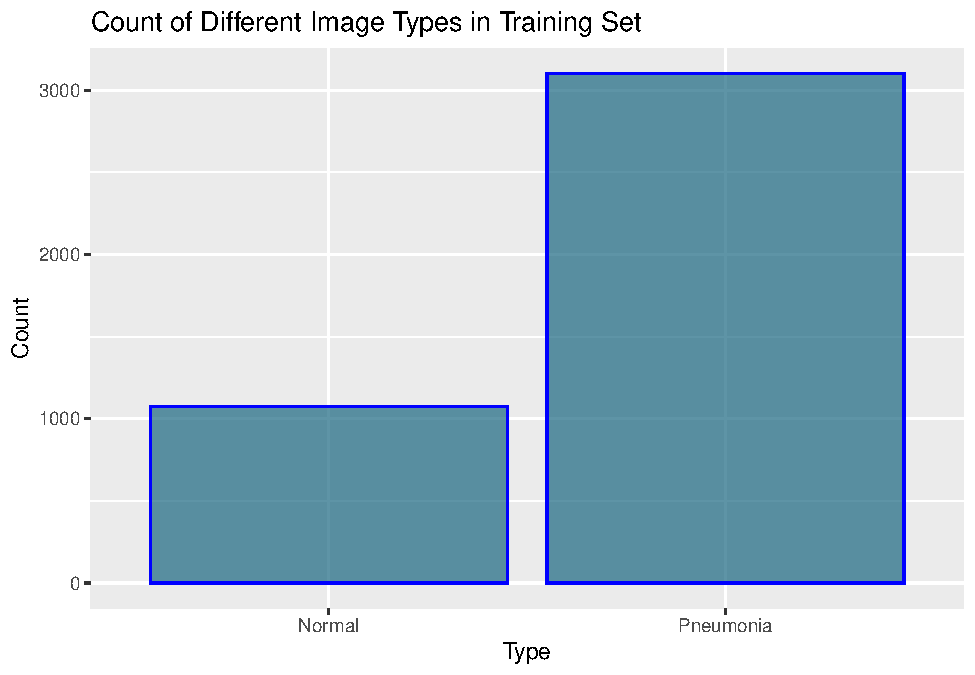
\includegraphics{report_files/figure-latex/unnamed-chunk-4-1.pdf}

\begin{Shaded}
\begin{Highlighting}[]
\NormalTok{patients2<-patients }\OperatorTok\StringTok{ }\KeywordTok{filter}\NormalTok{(lesion_type }\OperatorTok{!=}\StringTok{ "Unknown"}\NormalTok{)}

\KeywordTok{ggplot}\NormalTok{(patients2, }\KeywordTok{aes}\NormalTok{(}\DataTypeTok{x=}\NormalTok{patient_age, }\DataTypeTok{fill =}\NormalTok{ lesion_type)) }\OperatorTok{+}
\StringTok{  }\KeywordTok{geom_density}\NormalTok{(}\DataTypeTok{alpha =} \FloatTok{0.2}\NormalTok{) }\OperatorTok{+}
\StringTok{  }\KeywordTok{labs}\NormalTok{(}\DataTypeTok{x =} \StringTok{"Patient Age"}\NormalTok{, }\DataTypeTok{title =} \StringTok{"Density Plot of Patient Ages by Lesion Type"}\NormalTok{)}
\end{Highlighting}
\end{Shaded}

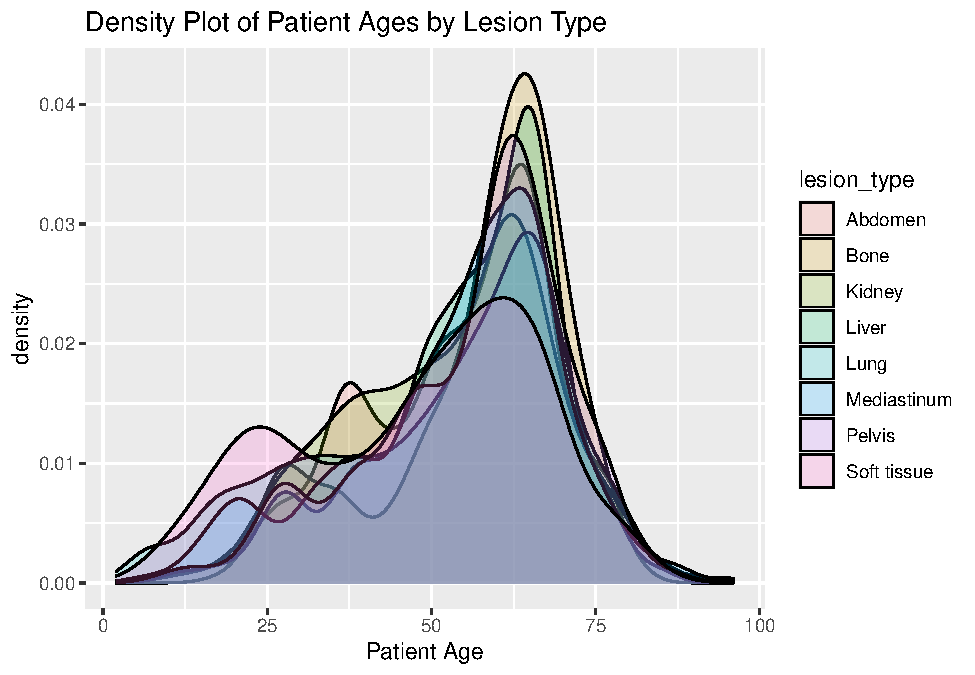
\includegraphics{report_files/figure-latex/unnamed-chunk-5-1.pdf}

\begin{Shaded}
\begin{Highlighting}[]
\KeywordTok{ggplot}\NormalTok{(}\DataTypeTok{data =}\NormalTok{ patients, }\KeywordTok{aes}\NormalTok{(}\DataTypeTok{x =}\NormalTok{ lesion_type, }\DataTypeTok{fill=}\NormalTok{Gender)) }\OperatorTok{+}
\StringTok{  }\KeywordTok{geom_bar}\NormalTok{() }\OperatorTok{+}
\StringTok{  }\KeywordTok{coord_flip}\NormalTok{()}\OperatorTok{+}
\StringTok{  }\KeywordTok{scale_fill_manual}\NormalTok{(}\DataTypeTok{values =} \KeywordTok{c}\NormalTok{(}\StringTok{"#69b3a2"}\NormalTok{, }\StringTok{"#404080"}\NormalTok{)) }\OperatorTok{+}
\StringTok{  }\KeywordTok{labs}\NormalTok{(}\DataTypeTok{x =} \StringTok{"Legion Type"}\NormalTok{, }\DataTypeTok{title =} \StringTok{"Bar Plot of Lesion Type by Gender"}\NormalTok{)}
\end{Highlighting}
\end{Shaded}

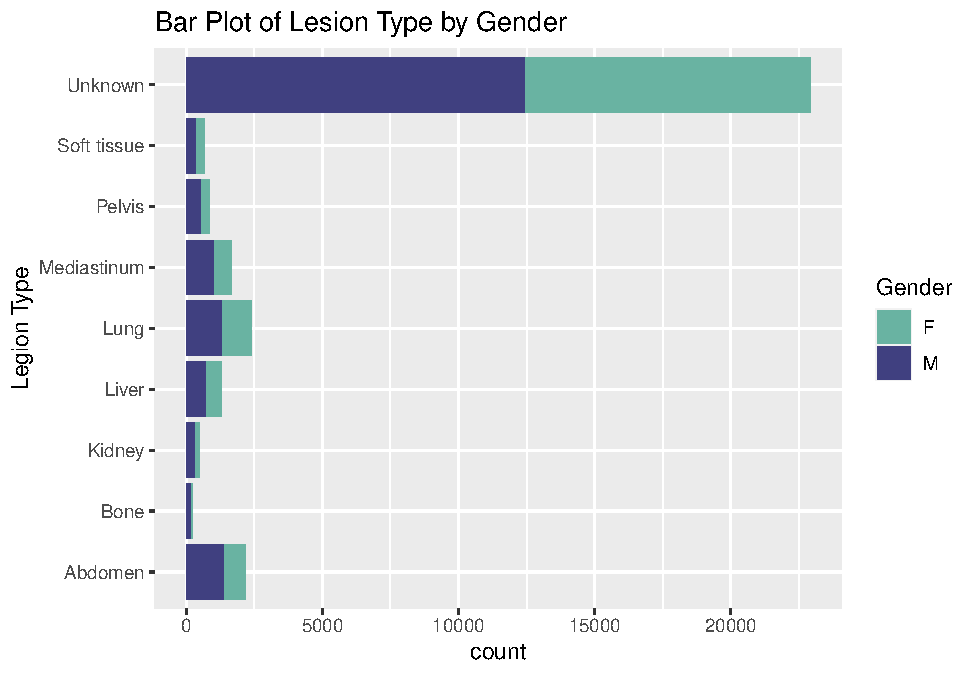
\includegraphics{report_files/figure-latex/unnamed-chunk-6-1.pdf}

\begin{Shaded}
\begin{Highlighting}[]
\NormalTok{patients2<-patients }\OperatorTok\StringTok{ }\KeywordTok{filter}\NormalTok{ (radius}\OperatorTok{<}\DecValTok{250} \OperatorTok{&}\StringTok{ }\NormalTok{lesion_type }\OperatorTok{!=}\StringTok{ "Unknown"}\NormalTok{)}

\KeywordTok{ggplot}\NormalTok{(}\DataTypeTok{data =}\NormalTok{ patients2, }\KeywordTok{aes}\NormalTok{(}\DataTypeTok{x =}\NormalTok{ radius,}\DataTypeTok{fill=}\NormalTok{lesion_type)) }\OperatorTok{+}
\StringTok{  }\KeywordTok{geom_density}\NormalTok{(}\DataTypeTok{alpha=}\FloatTok{0.2}\NormalTok{) }\OperatorTok{+}
\StringTok{  }\KeywordTok{labs}\NormalTok{(}\DataTypeTok{x =} \StringTok{"Radius"}\NormalTok{, }\DataTypeTok{title =} \StringTok{"Density Plot of Radius by Lesion Type"}\NormalTok{)}
\end{Highlighting}
\end{Shaded}

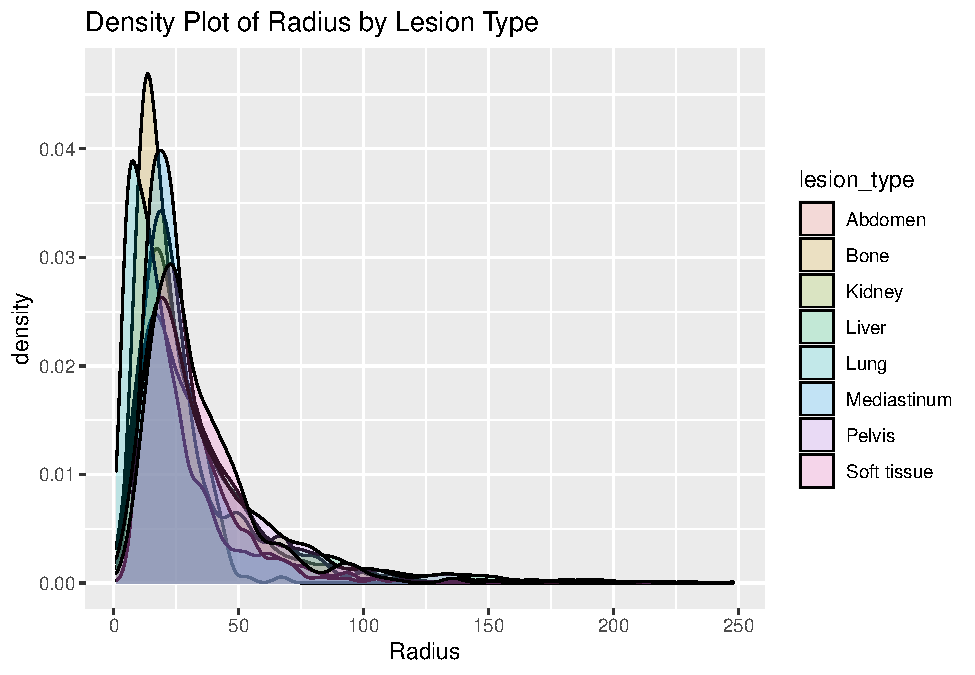
\includegraphics{report_files/figure-latex/unnamed-chunk-7-1.pdf}

\hypertarget{this-to-to-print-out-some-of-the-images-of-the-actual-lesions}{%
\subsection{This to to print out some of the images of the actual
lesions}\label{this-to-to-print-out-some-of-the-images-of-the-actual-lesions}}

-This needs to be changed, meant to have a box around where the legion
is but currently not working -Also planning to add multiple of these
types of images

\begin{Shaded}
\begin{Highlighting}[]
\NormalTok{image<-}\KeywordTok{gcs_get_object}\NormalTok{(objects}\OperatorTok{$}\NormalTok{name[[}\DecValTok{9}\NormalTok{]], }\DataTypeTok{saveToDisk=}\StringTok{"patient0.jpeg"}\NormalTok{, }\DataTypeTok{overwrite =} \OtherTok{TRUE}\NormalTok{)}
\end{Highlighting}
\end{Shaded}

\begin{verbatim}
## 2020-11-12 00:50:28 -- Saved archive/minideeplesion/000001_01_01/109.png to patient0.jpeg (200.9 Kb)
\end{verbatim}

\begin{Shaded}
\begin{Highlighting}[]
\NormalTok{img<-}\KeywordTok{image_read}\NormalTok{(}\StringTok{"patient0.jpeg"}\NormalTok{)}
\NormalTok{img<-}\KeywordTok{image_normalize}\NormalTok{(img)}

\KeywordTok{image_info}\NormalTok{(img)}
\end{Highlighting}
\end{Shaded}

\begin{verbatim}
## # A tibble: 1 x 7
##   format width height colorspace matte filesize density
##   <chr>  <int>  <int> <chr>      <lgl>    <int> <chr>  
## 1 PNG      512    512 Gray       FALSE        0 72x72
\end{verbatim}

\begin{Shaded}
\begin{Highlighting}[]
\NormalTok{image<-}\KeywordTok{ggdraw}\NormalTok{() }\OperatorTok{+}
\StringTok{  }\KeywordTok{draw_image}\NormalTok{(}
\NormalTok{    img, }\DataTypeTok{scale =} \DecValTok{1}
\NormalTok{  ) }\OperatorTok{+}\StringTok{ }\KeywordTok{geom_rect}\NormalTok{(}\KeywordTok{aes}\NormalTok{(}\DataTypeTok{xmin =} \DecValTok{0}\NormalTok{, }\DataTypeTok{xmax =} \DecValTok{20}\NormalTok{, }\DataTypeTok{ymin =} \DecValTok{0}\NormalTok{, }\DataTypeTok{ymax =} \DecValTok{20}\NormalTok{), }\DataTypeTok{alpha =} \DecValTok{1}\OperatorTok{/}\DecValTok{10}\NormalTok{,}\DataTypeTok{fill =} \StringTok{"red"}\NormalTok{)}
\NormalTok{image}
\end{Highlighting}
\end{Shaded}

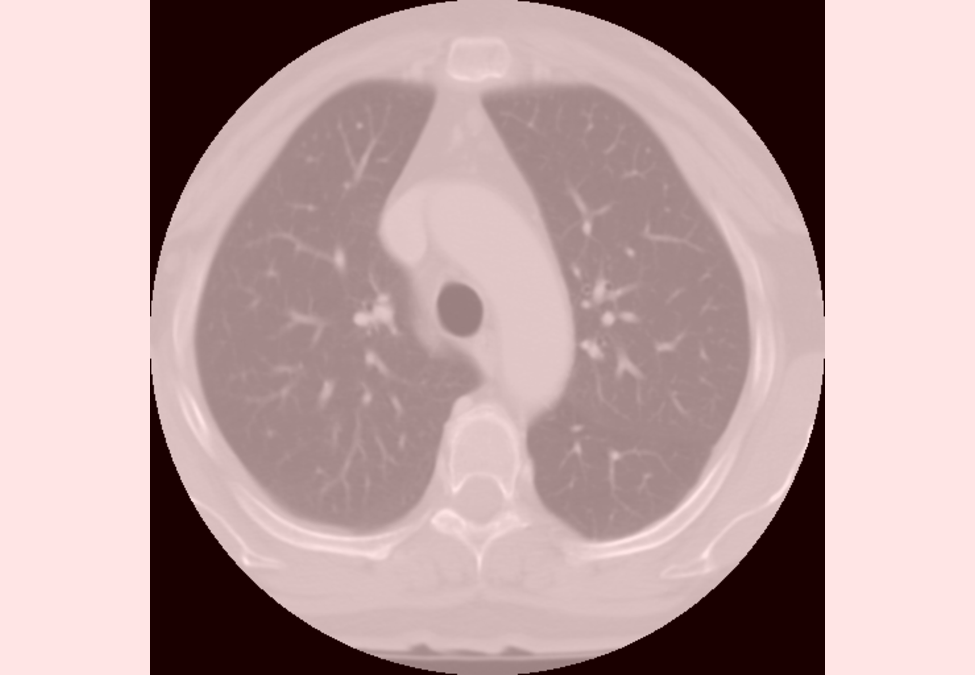
\includegraphics{report_files/figure-latex/unnamed-chunk-8-1.pdf}

\hypertarget{this-is-where-i-will-begin-my-work-with-spark-now-that-all-the-data-is-available-from-google-cloud-storage}{%
\subsection{This is where I will begin my work with Spark now that all
the data is available from Google Cloud
Storage}\label{this-is-where-i-will-begin-my-work-with-spark-now-that-all-the-data-is-available-from-google-cloud-storage}}

-This is not complete

\begin{Shaded}
\begin{Highlighting}[]
\CommentTok{#spark_install()}

\NormalTok{sc <-}\StringTok{ }\KeywordTok{spark_connect}\NormalTok{(}\DataTypeTok{master =} \StringTok{"local"}\NormalTok{, }\DataTypeTok{version =} \StringTok{"2.3"}\NormalTok{)}


\NormalTok{medical <-}\StringTok{ }\KeywordTok{copy_to}\NormalTok{(sc, medical_data)}
\NormalTok{images<-}\KeywordTok{copy_to}\NormalTok{(sc,objects )}
\NormalTok{medical}
\end{Highlighting}
\end{Shaded}

\begin{verbatim}
## # Source: spark<medical_data> [?? x 22]
##    file_name patient_index study_index series_id key_slice_index
##    <chr>             <dbl>       <dbl>     <dbl>           <dbl>
##  1 000001_0~             1           1         1             109
##  2 000001_0~             1           2         1              14
##  3 000001_0~             1           2         1              17
##  4 000001_0~             1           3         1              88
##  5 000001_0~             1           4         1              17
##  6 000002_0~             2           1         1             162
##  7 000002_0~             2           1         1             176
##  8 000002_0~             2           2         1              50
##  9 000002_0~             2           2         1              52
## 10 000002_0~             2           2         1              65
## # ... with more rows, and 17 more variables: measurement_coordinates <chr>,
## #   bounding_boxes <chr>, lesion_diameters_pixel <chr>,
## #   normalized_lesion_location <chr>, coarse_lesion_type <dbl>,
## #   possibly_noisy <dbl>, slice_range <chr>, spacing_mm_px <chr>,
## #   image_size <chr>, dicom_windows <chr>, patient_gender <chr>,
## #   patient_age <dbl>, train_val_test <dbl>, file_path <chr>,
## #   object_path <chr>, radius <chr>, lesion_type <chr>
\end{verbatim}

\begin{Shaded}
\begin{Highlighting}[]
\KeywordTok{spark_web}\NormalTok{(sc)}

\KeywordTok{spark_disconnect}\NormalTok{(sc)}
\end{Highlighting}
\end{Shaded}

\hypertarget{data-preprocessing-to-set-up-testing-and-training-sets-of-the-medical-images}{%
\subsection{Data Preprocessing To Set Up Testing and Training Sets of
the medical
images}\label{data-preprocessing-to-set-up-testing-and-training-sets-of-the-medical-images}}

-This is not complete

\begin{Shaded}
\begin{Highlighting}[]
\NormalTok{im <-}\StringTok{ }\KeywordTok{load.image}\NormalTok{(}\StringTok{"patient0.jpeg"}\NormalTok{) }\OperatorTok\StringTok{ }\KeywordTok{grayscale}\NormalTok{()}
\end{Highlighting}
\end{Shaded}

\begin{verbatim}
## Warning in grayscale(.): Image appears to already be in grayscale mode
\end{verbatim}

\begin{Shaded}
\begin{Highlighting}[]
\KeywordTok{plot}\NormalTok{(im)}
\end{Highlighting}
\end{Shaded}

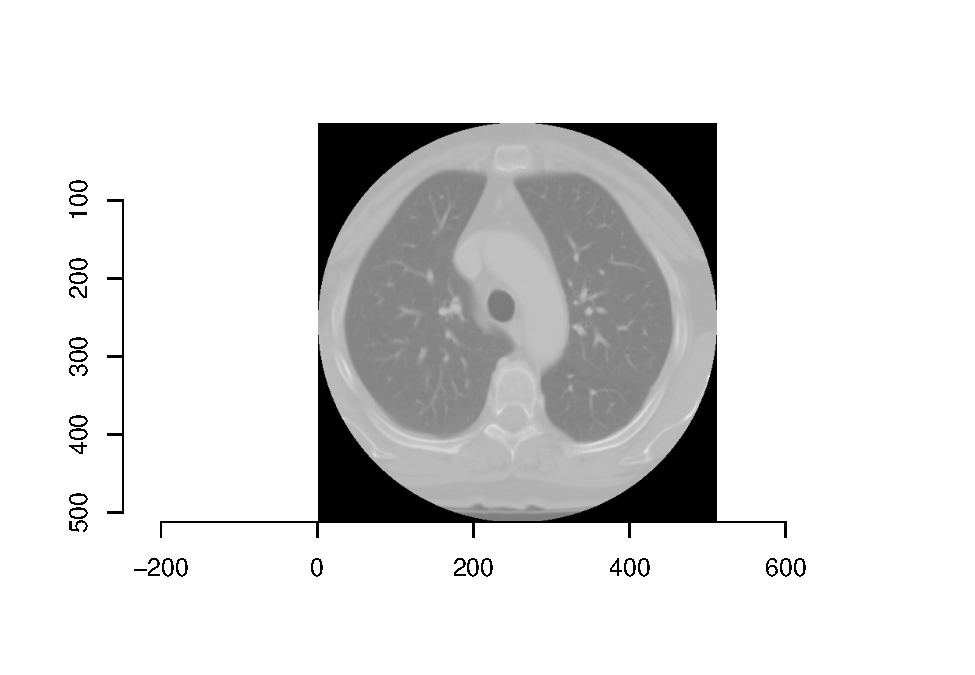
\includegraphics{report_files/figure-latex/unnamed-chunk-10-1.pdf}

\begin{Shaded}
\begin{Highlighting}[]
\KeywordTok{dim}\NormalTok{(im)}
\end{Highlighting}
\end{Shaded}

\begin{verbatim}
## [1] 512 512   1   1
\end{verbatim}

\begin{Shaded}
\begin{Highlighting}[]
\NormalTok{x<-}\KeywordTok{as.matrix}\NormalTok{(im)}
\end{Highlighting}
\end{Shaded}

\begin{Shaded}
\begin{Highlighting}[]
\KeywordTok{set.seed}\NormalTok{(}\DecValTok{123}\NormalTok{)}
\NormalTok{random <-}\StringTok{ }\KeywordTok{sample}\NormalTok{(}\DecValTok{1}\OperatorTok{:}\KeywordTok{nrow}\NormalTok{(all_images), }\FloatTok{0.8} \OperatorTok{*}\StringTok{ }\KeywordTok{nrow}\NormalTok{(all_images)) }\CommentTok{# 80%: training data, 20%: test data}
\NormalTok{train <-}\StringTok{ }\NormalTok{all_images[random, ] }
\NormalTok{train2<-}\StringTok{ }\NormalTok{train }\OperatorTok\StringTok{ }\KeywordTok{left_join}\NormalTok{(medical_data, }\DataTypeTok{by=} \KeywordTok{c}\NormalTok{(}\StringTok{"name"}\NormalTok{=}\StringTok{"object_path"}\NormalTok{))}

\NormalTok{test <-}\StringTok{ }\NormalTok{all_images[}\OperatorTok{-}\NormalTok{random, ]}
\NormalTok{test2<-}\StringTok{ }\NormalTok{test }\OperatorTok\StringTok{ }\KeywordTok{left_join}\NormalTok{(medical_data, }\DataTypeTok{by=} \KeywordTok{c}\NormalTok{(}\StringTok{"name"}\NormalTok{=}\StringTok{"object_path"}\NormalTok{))}
\CommentTok{#image2<-gcs_get_object(train$name[[1]], saveToDisk="patient1.jpeg", overwrite = TRUE)}
\end{Highlighting}
\end{Shaded}

\hypertarget{this-is-where-i-will-do-more-of-the-machine-learning-and-convolution-neural-netowrks-within-spark}{%
\subsection{This is where I will do more of the machine learning and
convolution neural netowrks within
Spark}\label{this-is-where-i-will-do-more-of-the-machine-learning-and-convolution-neural-netowrks-within-spark}}

\begin{Shaded}
\begin{Highlighting}[]
\CommentTok{# data_dir <- gs_data_dir("gs://medical_images/archive/minideeplesion") }
\CommentTok{# images <- list.files(data_dir, pattern = ".png", recursive = TRUE)}
\CommentTok{# length(images)}
\CommentTok{# }
\CommentTok{# classes <- list.dirs(data_dir, full.names = FALSE, recursive = FALSE)}
\CommentTok{# classes}
\CommentTok{# }
\CommentTok{# list_ds <- file_list_dataset(file_pattern = paste0(data_dir, "/*/*"))}
\CommentTok{# list_ds %>% reticulate::as_iterator() %>% reticulate::iter_next()}
\CommentTok{# list_ds}
\CommentTok{# }
\CommentTok{# get_label <- function(file_path) \{}
\CommentTok{#   parts <- tf$strings$split(file_path, "/")}
\CommentTok{#   parts[-2] %>% }
\CommentTok{#     tf$equal(classes) %>% }
\CommentTok{#     tf$cast(dtype = tf$float32)}
\CommentTok{# \}}
\CommentTok{# }
\CommentTok{# decode_img <- function(file_path, height = 224, width = 224) \{}
\CommentTok{#   }
\CommentTok{#   size <- as.integer(c(height, width))}
\CommentTok{#   }
\CommentTok{#   file_path %>% }
\CommentTok{#     tf$io$read_file() %>% }
\CommentTok{#     tf$image$decode_jpeg(channels = 3) %>% }
\CommentTok{#     tf$image$convert_image_dtype(dtype = tf$float32) %>% }
\CommentTok{#     tf$image$resize(size = size)}
\CommentTok{# \}}
\CommentTok{# }
\CommentTok{# preprocess_path <- function(file_path) \{}
\CommentTok{#   list(}
\CommentTok{#     decode_img(file_path),}
\CommentTok{#     get_label(file_path)}
\CommentTok{#   )}
\CommentTok{# \}}
\CommentTok{# }
\CommentTok{# labeled_ds <- list_ds %>% }
\CommentTok{#   dataset_map(preprocess_path, num_parallel_calls = tf$data$experimental$AUTOTUNE)}
\CommentTok{# }
\CommentTok{# labeled_ds %>% }
\CommentTok{#   reticulate::as_iterator() %>% }
\CommentTok{#   reticulate::iter_next()}
\end{Highlighting}
\end{Shaded}

\begin{Shaded}
\begin{Highlighting}[]
\CommentTok{# prepare <- function(ds, batch_size, shuffle_buffer_size) \{}
\CommentTok{#   }
\CommentTok{#   if (shuffle_buffer_size > 0)}
\CommentTok{#     ds <- ds %>% dataset_shuffle(shuffle_buffer_size)}
\CommentTok{#   }
\CommentTok{#   ds %>% }
\CommentTok{#     dataset_batch(batch_size) %>% }
\CommentTok{#     # `prefetch` lets the dataset fetch batches in the background while the model}
\CommentTok{#     # is training.}
\CommentTok{#     dataset_prefetch(buffer_size = tf$data$experimental$AUTOTUNE)}
\CommentTok{# \}}
\CommentTok{# }
\CommentTok{# model <- keras_model_sequential() %>% }
\CommentTok{#   layer_flatten() %>% }
\CommentTok{#   layer_dense(units = 128, activation = "relu") %>% }
\CommentTok{#   layer_dense(units = 128, activation = "relu") %>% }
\CommentTok{#   layer_dense(units = 5, activation = "softmax")}
\CommentTok{# }
\CommentTok{# model %>% }
\CommentTok{#   compile(}
\CommentTok{#     loss = "categorical_crossentropy",}
\CommentTok{#     optimizer = "adam",}
\CommentTok{#     metrics = "accuracy"}
\CommentTok{#   )}
\CommentTok{# }
\CommentTok{# model %>% }
\CommentTok{#   fit(}
\CommentTok{#     prepare(labeled_ds, batch_size = 32, shuffle_buffer_size = 1000),}
\CommentTok{#     epochs = 5,}
\CommentTok{#     verbose = 2}
\CommentTok{#   )}
\end{Highlighting}
\end{Shaded}

\begin{Shaded}
\begin{Highlighting}[]
\CommentTok{# trial<-flow_images_from_directory(directory=data_dir,}
\CommentTok{#                            generator = image_data_generator(rescale=1/255),}
\CommentTok{#                            target_size=c(256,256), color_mode = "grayscale")}
\CommentTok{# trial}
\CommentTok{# data_dir <- gs_data_dir("gs://medical_images/archive/minideeplesion/000002_02_01/044.png") }
\CommentTok{# trial<-image_load(path="gs://medical_images/archive/minideeplesion/000002_02_01", grayscale=TRUE)}
\end{Highlighting}
\end{Shaded}

\bibliographystyle{agsm}
\bibliography{bibliography.bib}

\end{document}
